\documentclass[11pt,a4paper]{report}

\setlength\textwidth{145mm}
\setlength\textheight{247mm}
\setlength\oddsidemargin{15mm}
\setlength\evensidemargin{15mm}
\setlength\topmargin{0mm}
\setlength\headsep{0mm}
\setlength\headheight{0mm}
\let\openright=\clearpage

\usepackage[czech]{babel}
\usepackage{lmodern}
\usepackage[T1]{fontenc}
\usepackage{textcomp}

\usepackage[utf8]{inputenc}

\usepackage{stddoc}


\renewcommand{\vec}{\boldsymbol}
\def\endl{\\[3mm]}
\newcommand*\colvec[3][]{
	\begin{pmatrix}
		\ifx \relax#1 \relax
		\else #1\\
		\fi
		#2 \\ #3
	\end{pmatrix}
}


\makeatletter
\def\thmheadbrackets#1#2#3{%
	\thmname{#1}\thmnumber{\@ifnotempty{#1}{ }\@upn{#2}}%
	\thmnote{{ \the\thm@notefont[#3]}}}
\makeatother

\newtheoremstyle{theorem}			% name
{\topsep}						% Space above
{\topsep}						% Space below
{\normalfont}					% Body font
{}								% Indent amount
{\bfseries}						% Theorem head font
{.}								% Punctuation after theorem head
{1em}							% Space after theorem head
{\thmheadbrackets{#1}{#2}{#3}}	% theorem head spec

%\renewenvironment{proof}{{\noindent\bfseries Důkaz.}}{\qed}

\theoremstyle{theorem}
\newtheorem{theorem}{Věta}[section]
\newtheorem{claim}{Tvrzení}[section]
\newtheorem{example}{Příklad}
% The additional parameter [section] restarts the theorem counter at every new section.
\newtheorem{corollary}{Důsledek}[theorem]
% An environment called corollary is created, the counter of this new environment will be reset every time a new theorem environment is used.
\newtheorem{lemma}[theorem]{Lemma}
% In this case, the even though a new environment called lemma is created, it will use the same counter as the theorem environment.
\newtheorem*{observation}{Pozorování}
\newtheorem*{recap}{Opakování}

\theoremstyle{remark}
\newtheorem*{remark}{Poznámka}
\newtheorem*{solution}{Řešení}
\newtheorem*{convention}{Konvence}
% The syntax of the command \newtheorem* is the same as the non-starred version, except for the counter parameters. In this example a new unnumbered environment called remark is created.

\theoremstyle{definition}
\newtheorem{definition}{Definice}[section]



\begin{document}
	
	\pagenumbering{gobble}
	
	\section*{Magnetické pole}
		
		\paragraph*{Disclaimer.} Obrázky nejsou mojí tvorbou, jsou vypůjčeny ze souboru seminářů od prof. Kulhánka.
		
		Podobnou roli Gaussovu zákonu elektrostatiky v magnetostatice hraje zákon Ampérův. Jedná se o velice mocný výpočetní nástroj, který může z výpočtu, který by byl jinak pracný, učinit jednořádkovou trivialitu. Má však stejné hranice jako v elektrostatice zákon Gaussův, což jsou symetrie. Apérův zákon nám značně zjednodušuje práci v magnetostatických polích, ale pouze v případě symetrických úloh. Pro obecné úlohy musíme použít vzathů obecnějších, jako například Biot-Savartův zákon. Takovými nepřijemnostmi my se však dnes zabývat nebudeme a vystačíme si s Ampérovým zákonem, jakožto s jednou z Maxwellových rovnic%
			\footnote{V Maxwellových rovnicích bychom tento zákon našli ještě rozšířený o časovou derivaci elektrického pole, kterou tam přidal práve až Maxwell. Jelikož my se však zabýváme čistě magnetostatikou (časové derivace polí jsou tedy nulové), nemusíme tento elektrodynamický vliv do našich výpočtů zahrnovat.}
		v integrálním tvaru.
		
		\begin{figure}[h!]
			\begin{center}
				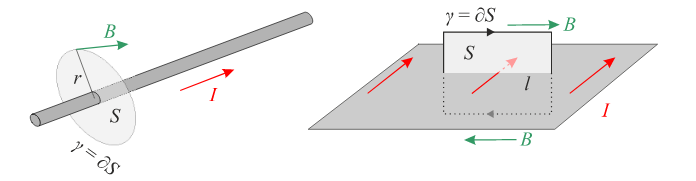
\includegraphics[width=0.9\linewidth]{img/1.png}
				\caption{Ilustrační obrázek k příkladům \ref{1} a \ref{3}}
			\end{center}
		\end{figure}
		
		\begin{example}
			\label{1}
			Určete velikost magnetického pole v okolí dlouhého přímého vodiče protékaného elektrickým proudem $I$.
		\end{example}
		\begin{solution}
			Z Maxwellových rovnic víme
			\begin{align*}
				\div \vec B &= 0,
			&
				\oint_S \vec B \cdot \d \vec S &= 0.
			\end{align*}
			Můžeme tedy učinit úvahu, že siločáry magnetického pole jsou vždy uzavřené (nebo nekonečné). Mohli bychom tedy kreslit libovolný tvar magnetického pole okolo vodiče, ale rotační symetrie válcového vodiče nám diktuje jediný možný tvar takovýchto uzavřených siločar a to jsou kružnice.%
				\footnote{Tuto úvahu není samozřejmě třeba pokaždé dělat, člověk toto zná již ze střední školy z Ampérova zákona pravé ruky. Zde je však pouze pěkné vysvětlení. Ampérovo pravidlo pravé ruky dále udává směr otáčení těchto siločar, což již vyplývá kvalitativně z Biot-Savartova zákona.}
			Napišme tedy Ampérův zákon v integrálním tvaru
			\begin{align*}
				\oint_\gamma \vec B \cdot \d \vec \l &= \mu_0 I,
			\end{align*}
			kde za integrační křivku (vizte obrázek 1 vlevo) bereme výhodně kružnici souosou s vodičem. Výhodnost volby spočívá v tom, že, jak jsme právě určili, takto zvolená křivka bude mít v každém bodě tečný vektor kolineární s vektorem magnetické indukce. Původně složitý integrál vektorového pole se nám zjednoduší na integraci skalární funkce a můžeme tak psát
			\begin{align*}
				\oint_\gamma \vec B \cdot \d \vec \l = \oint_\gamma B \; \d \l = B \oint_\gamma \; \d \l = B\l = B 2\pi r.
			\end{align*}
			Můžeme tedy psát rovnou výsledek
			\begin{align*}
				B 2 \pi r &= \mu_0 I,
			\\
				B &= \frac{\mu_0 I}{2\pi r}.
			\end{align*}
			Přidáním vektorového charakteru magnetického pole do výsledku, který jsme získali úvahou, můžeme psát
			\begin{align*}
				\Aboxed{B &= \frac{\mu_0 I}{2\pi r} \vec e_\varphi,}
			\end{align*}
			kde $\vec e_\varphi$ je jednotkový vektor ve směru růstu polární souřadnice $\varphi$.
		\end{solution}
		
		\begin{example}
			\label{2}
			Vypočítejte indukci magnetického pole buzeného dvěma přímými nekonečně dlouhými rovnoběžnými vodiči, které jsou od sebe vzádelny $d$ a teče jimi proud $I$ stejným směrem ve vzálenosti $a$ od prvního vodiče na spolčné kolmé spojici obou vodičů. Vodiče jsou umístěny ve vakuu. 
		\end{example}
		\begin{solution}
			Díky námi odvozenému vztahu pro magnetické pole (tzv. magnetickou indukci) v okolí přímého vodiče se jedná téměr o pouhé dosazení do vzorce. Pouze tentokrát se jedná o situaci, kdy máme dva vodiče souhlasného proudu, takže provedeme superposici příspěvků od obou vodičů. Z naší předchozí úvahy (Ampérovo pravidlo pravé ruky) pro jednotlivé přímé vodiče vyplývá, že směry jimi generovaných magnetických polí budou opačné, tudíž musíme jejich příspěvky odečíst. Dostáváme tedy
			\begin{align*}
				B &= B_1 + B_2 = \frac{\mu_0 I}{2\pi a} - \frac{\mu_0 I}{2\pi(d-a)} = \frac{\mu_0 I}{2\pi} \( \frac 1a - \frac{1}{d-a} \).
			\end{align*}
		\end{solution}
	
		\begin{example}
			\label{3}
			Určete magnetické pole v okolí plochy protékané elektrickým proudem.
		\end{example}
		\begin{solution}
			V případě roviny protékané proudem, bude magnetické pole (znovu dle Ampérova pravidla pravé ruky) rovnoběžný s plochou, jak je znázorněno na obrázku 1 vpravo. Zvolme tedy jako integrační křivku obdélník kolmý na rovinu a směr proudu. Díky tomu se nám zjednoduší integrál na
			\begin{align*}
				\oint_\gamma \vec B \cdot \d \vec \l = 2 \mathcal I_\parallel + 2 \mathcal I_\perp,
			\end{align*}
			kde $\mathcal I_\parallel$ je úsek integrace rovnoběžný s plohou (a tedy i se siločárami pole) a $\mathcal I_\perp$ je kolmý úsek. Díky vlastnostem skalárního součinu $\vec B \cdot \d \l$ s takto definovanou křivkou můžeme tedy psát
			\begin{align*}
				2 \mathcal I_\parallel + 2 \mathcal I_\perp = 2B\l + 0 = 2B\l.
			\end{align*}
			Můžeme tedy psát již závěr, jedinou změnou bude vyjádření celkového protékaného proudu pomocí proudové hustoty jako $I = i \l$. Konečně tedy
			\begin{align*}
				2B\l &= \mu_0 i \l,
			\\
				B &= \frac{\mu_0 i}{2}.
			\end{align*}
			Přidáme-li do výsledku námi zvážený vektorový charakter, dostáváme výsledek ve tvaru
			\begin{align*}
				\vec B = \left\{ \begin{matrix}
					\vec e_x (\mu_0 i)/2, & \text{pro } z > 0,
				\\
					- \vec e_x (\mu_0 i)/2, & \text{pro } z < 0,
				\end{matrix} \right.
			\end{align*}
			kde $\vec e_x$ je znovu jednotkový vektor ve směru růstu, tentokrát kartézské, souřadnice $x$.
		\end{solution}
		
		\begin{example}
			\label{4}
			Určete magnetické pole uvnitř i vně vodiče, jehož průřezem protéká konstantní proudová hustota. Vodič je natolik dlouhý, že lze zanedbat okrajové efekty.
		\end{example}
		\begin{figure}[h!]
			\begin{center}
				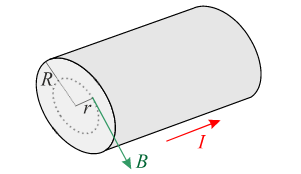
\includegraphics[width=0.5\linewidth]{img/2.png}
				\caption{Ilustrační obrázek k příkladu \ref{4}}
			\end{center}
		\end{figure}
		\begin{solution}
			Zde vlastně dořešíme první úlohu i uvnitř vodiče, přičemž ke konsolidaci využijeme již dříve získáného vztahu pro vnější pole. Tentokrát však při využití Ampérovy věty využijeme poměrného proudu $I_r$, který (jak je vidět z obrázku 2) omezuje celkový proud $I$ volbou integrační kružnice o poloměru $r<R$ ve stejném poměru jako poměry uzavřených ploch, tedy $I_r = I (S_r/S_R)$.
			\begin{align*}
				\oint_\gamma \vec B \cdot \d \vec \l &= \mu_0 I_r,
			\\
				B 2 \pi r &= \mu_0 I \frac{S_r}{S_R},
			\\
				B 2 \pi r &= \mu_0 I \frac{r^2}{R^2},
			\\
				B &= \mu_0 I \frac{r}{2 \pi R^2}.
			\end{align*}
			Spojíme-li výsledek s řešením prvního příkladu, můžeme pro magnetické pole generované vodičem psát
			\begin{align*}
				B = \left\{ \begin{matrix}
					\mu_0 I \frac{r}{2 \pi R^2}, & \text{pro } r \leq 0,
				\\[2mm]
					\frac{\mu_0 I}{2\pi r}, & \text{pro } r > R.
				\end{matrix} \right.
			\end{align*}
		\end{solution}
	
	
	
	
\end{document}